\section{Software arkitektur}

\subsection{Fokuspunkter}

\begin{itemize}
	\item Redegøre for begrebet softwarearkitektur.
	\item Giv et eksempel på en typisk softwarearkitektur og dens anvendelse?
	\item Hvordan udarbejdes en software arkitektur?
	\item Hvordan dokumenteres en software arkitektur?
\end{itemize}

\subsection{Redegør for begrebet softwarearkitektur}
\textit{''The highest-level breakdown of a system into its parts; the decisions that are hard to change; ...  and, in the end, architecture boils down to whatever the important stuff is.''}

\subsubsection{Hvad er en software arkitektur?}
Den højeste abstraktion.

\begin{itemize}
	\item Fokuserer på de større elementer og komponenter.
	\begin{itemize}
		\item Hvordan er de organiserede.
		\item Hvordan interagerer de?
		\item Er der nogle problematiske områder? (Areas of concern).\todo{nøjagtig formulering?}
	\end{itemize}
	\item Software Design er en realisering af arkitekturen bag.
	\item Arkitekturen viser de elemter som er svære at ændre.\todo{svære hvordan?}
	\item Viser også de elemter der er de vigtigste.
\end{itemize}

\subsubsection{Hvorfor er det vigtigt?}
Med komplekse systemer er det vigtigt at have et solidt fundament.

\begin{itemize}
	\item Der er følgende risici uden en arkitektur:
	\begin{itemize}
		\item Hovedscenarier kan overses.\todo{Defineres disse ikke FØR arkitekturen?}
		\item Almindelige problemer bliver overset.\todo{igen, hvorfor?}
		\item At værdsætte fremtidige konsekvenser på baggrund af afgørende beslutninger.\todo{føles som øregas}
		\item Uden en arkitektur, står man let med et monolithic program (big ball of mud), dvs. uden egentlig struktur og under-elementer.
	\end{itemize}
\end{itemize}

\subsubsection{Generelle overvejselser}
\begin{itemize}
	\item \textbf{Applikationstype} - Mobile app, web app osv.
	\item \textbf{Deployment strategi} - Distribueret/ikke distribueret, runtime kørsel, mnætværksinfrastruktur.
	\item \textbf{Teknologier} - Protokoller, Sprog, etc - Hvilke skal i bruges?
	\item \textbf{Quality attributter} - Kvalitet af systemet.
	\begin{itemize}
		\item Conceptual integrity.\todo{what is?}
		\item Maintainablity.
		\item Reusability.
		\item Performance.
		\item Security.
		\item Scalability.
		\item Reliability.
	\end{itemize}
	\item \textbf{Design kvalitet}
	\begin{itemize}
		\item Supportability.
		\item Testability.
	\end{itemize}
\end{itemize}

\subsubsection{Architectural Styles}
Ligesom design patterns, findes der også patterns af arkitekturer, eller styles.
En arkitektur stil definerer en familie af systemer med ens struktur, navne af komponenter og connectors og med restriktioner omkring hvordan disse kan forbindes. De blandes ofte (på sammen måde som design patterns) - der bruges næsten aldrig kun én style.

\paragraph{Typer af styles (almindelige)}

\todo{savner forklaring af nogle de nedstående...}
\begin{itemize}
	\item Client/Server.\\
	Serveren kører et eller flere programmer, som deler deres ressourcer med klienter.
	\item Component based.
	\item Domain Driven Design.
	\item Layered - Den mest udbredte. Denne gives der eksempel på.
	\item Message bus.
	\item N-tier/3-Tier.\\
	En Client/server arkitektur hvor presentation, apllikation og processering er separeret. Tier (lag) opdeling. Den mest bruger er 3-tier.
	\item Object Oriented.
	\item Service oriented.\\
	Det samme som Client/server blot med flere servers.
	
\end{itemize}


\subsection{Giv et eksempel på en typisk softwarearkitektur og dens anvendelse}

\subsubsection{Layer}
\begin{itemize}
	\item Et layer er en grovkornet gruppering af: \textit{klasser, packages, og subsystemer}.
	\item Sørger for koblingsgraden i et system.\todo{hvordan ''sørger'' den for det?}
	\item Organisering af lag:
	\begin{itemize}
		\item Højere lag kalder funktioner i lavere lag.
		\item Lavere lag må ikke kalde på funktioner i højere lag. Lavere lag må dog godt notificere højere lag omkring hendelser med f.eks. observer pattern eller call-back funktions pointere (events).
	\end{itemize}
	\item Layer vs Tier - Layer er en \textbf{logisk separering}, hvorimod Tier er en repræsentation af den \textbf{fysiske seaparering}.
\end{itemize}

\paragraph{Fordele ved Layer}
\begin{itemize}
	\item Separation af ansvar (SRP).
	\begin{itemize}
		\item Separation af applikationsspecifik logik fra generel logik.
		\item Separation af høj niveau fra lav-niveau logik.
	\end{itemize}
	\item Reducerer kobling og afhængigheder.
	\item Større samhørighed.
	\item Højt potentiale for genbrug.
	\item Forholdsvist let at forstå/gennemskue.
	\item \textbf{Fremmer parallel udviking} da systemet bliver delt op i logiske segmenter.
	\item Et lag kan udskriftes hvis der er brugt interface baseret programmering.
\end{itemize}

\paragraph{Eksempel på layers}
Figur~\ref{fig:guiblldab} viser hvordan en layeropdelt arkitektur kunne se ud for et system som skal have en GUI og Database med et Business Logik niveau imellem.

\begin{figure}[h]
	\centering
	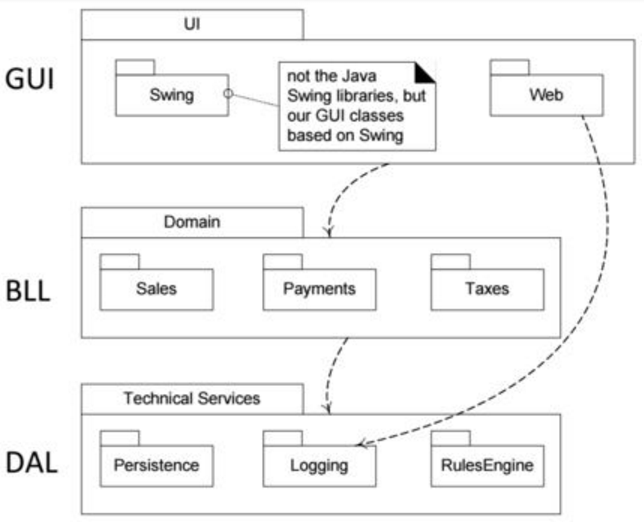
\includegraphics[width=0.7\linewidth]{figs/guiblldal}
	\caption{Arkitektur for et system med GUI, BLL og DAB logik.}
	\label{fig:guiblldab}
\end{figure}

Ligeledes kan man på figur~\ref{fig:osimodel} se den samme lagdeling i netværks modellen OSI\footnote{OSI: Open Systems Interconnection.}, som viser hvordan lagene imellem bruger hinanden.

\begin{figure}[h]
	\centering
	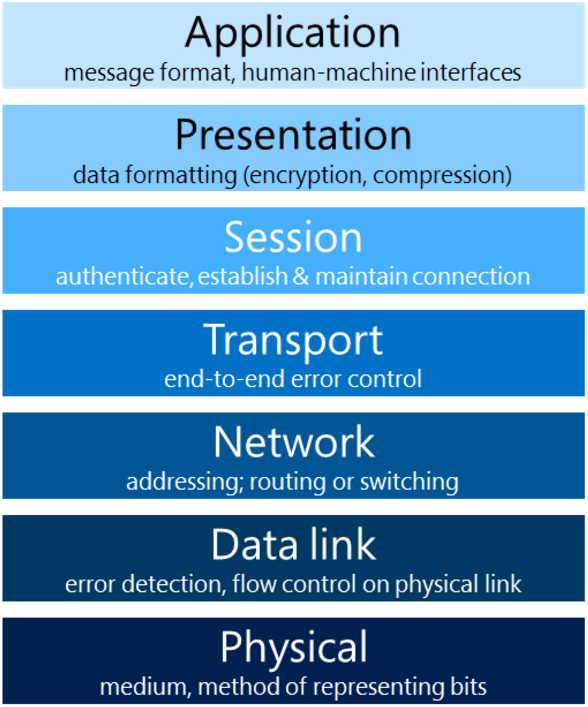
\includegraphics[width=0.5\linewidth]{figs/osimodel}
	\caption{Netværksarkitektur, Open Systems Interconnection Model (OSI model).}
	\label{fig:osimodel}
\end{figure}

\subsection{Hvordan udarbejdes en software arkitektur}
Der findes flere værktøjer:

\begin{itemize}
	\item ROPES: \textbf{R}apid \textbf{O}bject-oriented \textbf{P}rocess for \textbf{E}mbedded \textbf{S}ystems.\\
	Som navnet antyder er det primært til embedded software.
	\begin{itemize}
		\item Har 3 faser:
		\begin{itemize}
			\item Architectural.
			\item Mechanistic.
			\item Detailed Design (implementation).
		\end{itemize}
	\end{itemize}
	\item Iterativ (den vi mest bruger)
	\begin{itemize}
		\item 5 punkter, hvor de sidste 4 gentages iterativt, illustreret i figur~\ref{fig:arc_ite} og videre beskrevet i afsnit~\ref{sec:arc_ite}.
		\begin{enumerate}
			\item Identify architecture objectives.
			\item Identify key scenarios.
			\item Create application overview.
			\item Identify key issues.
			\item Define candidate solutions.
		\end{enumerate}
	\end{itemize}
\end{itemize}

\begin{figure}[h]
	\centering
	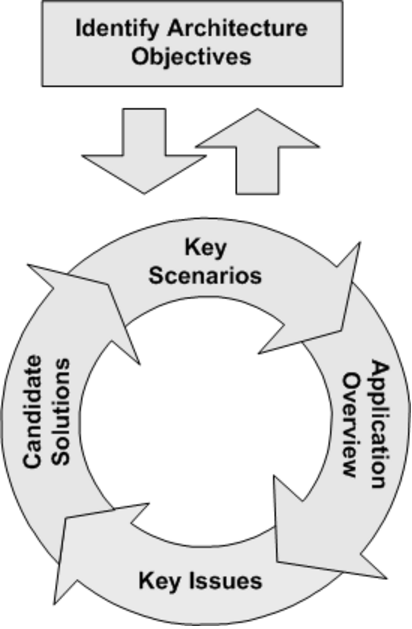
\includegraphics[width=0.35\linewidth]{figs/arc_ite}
	\caption{Process for iterativ arkitekturudvikling.}
	\label{fig:arc_ite}
\end{figure}

\subsubsection{Brug af Iterativ process}\label{sec:arc_ite}
Følgende trin anvendes i udvikling af produkt med iterativ projekt.

\paragraph{Identify Architecture Objectives}
\begin{itemize}
	\item Klare mål hjælper med at fokusere på arkitekturen og løse de konkrete probelmer i designet.
	\item Identificer arkitektur mål fra start.
	\item Identificer hvem der skal bruge arkitekturen.\todo{user bruger gui, tekniker bruger dab? like that?}
	\item Identificer dine begrænsninger.
\end{itemize}

\paragraph{Identify Key Scenarios}
\begin{itemize}
	\item Brug hovedscenarier til at fokusere dit design på hvad der betyder mest, og evaluer arkitektur kandidater herpå når de er klar.
	\item Hovedscenarier kan defineres som et scenarie der overholder en eller flere af følgende kriterier:
	\begin{itemize}
		\item Repræsenterer et betydeligt ukendt område eller et område af betydelig risiko.\todo{præcis mening?}
		\item Referere til en arkitektonisk vigtig use case.\todo{præcisering, tak}
		\item Repræsenterer bindeledet mellem en kvalitets attribut og funktionalitet.\todo{hvordan kommer kvalitet ind i use cases? accepttest lykkes?}
		\item Repræsenterer et tradeoff mellem kvalitets attributter. \today{how?}
	\end{itemize}
\end{itemize}

\paragraph{Create Application Overview}
\begin{itemize}
	\item Identificer:
	\begin{itemize}
		\item Applikations type.\todo{app, program console app what?}
		\item Deployment arkitektur. \todo{hvordan vi distribuere systemet?}
		\item Arkitektur style (type). \todo{means woot?}
		\item Teknologier. \todo{det valg af protocol etc?}
	\end{itemize}
\end{itemize}

Her forbindes dit design til den virkelige verden hvor applikationen operere. \todo{hvordan opstår denne forbindelse?}

\paragraph{Identify Key Issues}
Identificer de største problemer baseret på kvalitets attributter og crosscutting concerns. Begge nævn herunder.

\begin{itemize}
	\item \textbf{Kvalitets attributter}\\
	repræsentere områder af bekymring der kan have potentielle følger på tværs af lag.
	\begin{itemize}
		\item System kvalitet.\\
		Den generelle kvalitet for systemet som hvor godt/nemt er det at supporte/teste.
		\item Run-time kvalitet.\\
		Kvaliteten af systemet der gives til udtryk run-time, som performance og scalability.
		\item Design kvalitet.\\
		Kvaliteten der reflekteres i designet af systemet, som flexibilitet og genbrugelighed.
		\item Bruger kvalitet.\\
		Hvor godt/nemt systemet er at bruge.
	\end{itemize}
	\item \textbf{Crosscutting concerns}
	\begin{itemize}
		\item Grænseflader.
		\item Valg af metoder til Authentication, Cacging, Communikation etc.
	\end{itemize}
\end{itemize}

\paragraph{Define Candidate Solutions}
Skab en prototype der udvikler og forbedre løsningen og evaluer denne mod hovedscenarierne, problemerne og deployment begrænsningerne, før næste iteration af arkitekturen begyndes.

\begin{itemize}
	\item Få de største risici af vejen først.
	\item Lav iterative arkitekturelle tests der beviser at hver iteration er bedre end den forrige.
\end{itemize}

\subsection{Hvordan dokumenteres en software arkitektur}
Ved dokumentering af software arkitektur taler vi om to ting:
\begin{itemize}
	\item UML.
	\item n+1.
\end{itemize}

\subsubsection{UML}
Ved design af arkitektur anvendes tre nye UML diagramtyper:

\begin{itemize}
	\item Package diagrammer.\\
	Inderholder packages...\todo{som præcis er?}
	\item Deployment diagrammer.\\
	Indeholder Nodes...\todo{som er!?}
	\item Komponent diagrammer.\\
	Indeholder Komponenter...\todo{JESUS FUCK, HVAD ER DE HER TING!?}
\end{itemize}

Disse bruges sammen med de allerede kendt størrelser:

\begin{itemize}
	\item Task diagrammer, som udarbejdes vha. UML klassediagrammer.
	\item Aktivitets diagrammer.
	\item Klassediagrammer.
	\item Sekvens diagrammer.
\end{itemize}

\subsubsection{N+1}
Da der findes utallige måder at illustrere et system på, er n+1 (også kaldet 4+1), en bredspektret og mere struktureret måde at uddele forskellig funktionalitet i forskellige views.

Man behøver dog ikke bruge/vise alle views!

\begin{figure}[H]
	\centering
	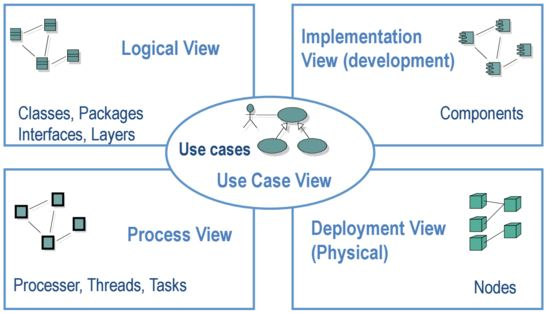
\includegraphics[width=0.8\linewidth]{figs/nplusoneview}
	\caption{De forskellige N+1 views.}
	\label{fig:nplusoneview}
\end{figure}

I forhold til hvilke diagrammer der bruges til de forskellige views, så viser figur~\ref{fig:nplusonedia} hvilke der kan bruges hvor.

\begin{figure}[H]
	\centering
	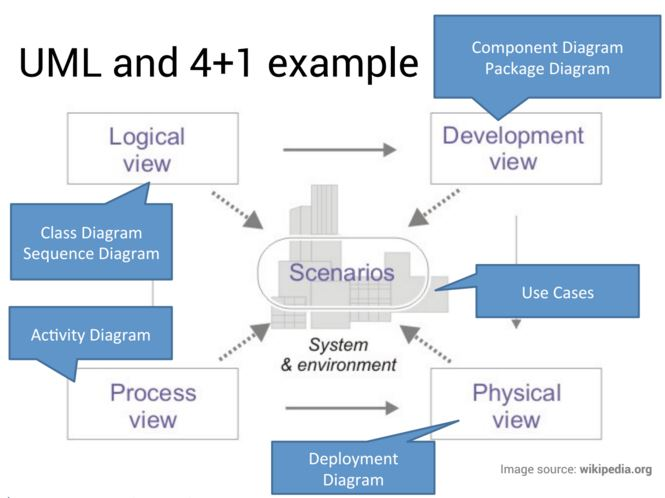
\includegraphics[width=0.8\linewidth]{figs/nplusonedia}
	\caption{De forskellige N+1 views.}
	\label{fig:nplusonedia}
\end{figure}

De fire views designes ud fra forskellige scenarier der udgør de 5. view “Scenarier”. Disse er som regel systemets use cases.\\

De fire views som er vist i figur~\ref{fig:nplusoneview} er så:
\begin{itemize}
	\item \textbf{Logical view}\\
	Systemets logik - hvordan kommunikere de forskellige klasser og komponenter.
	\item \textbf{Process view}\\
	Systemets performance - forholder sig til concurrency problemer og viser hvor der kan opstå problemer med parallelitet.
	\item \textbf{Development view}\\
	Systemets afhængigheder - fortæller hvordan de forskellige pakker/komponenter i systemet bliver ramt af ændring fra hinanden.
	\item \textbf{Physical view}\\
	System lokalisering - hvor er de forskellige delsystemet og hvor skal der implementeres kommunikation.
\end{itemize}